%!TEX root = ../memoire.tex

\chapter{Implémentation et évaluation du système}\label{eval}

Au chapitre précédent, nous avions extraits des informations précieuses de VerbNet à l'aide de scripts Python. Nous avons ainsi fait usage de ces informations en les implémentant dans GenDR. Ce chapitre est séparé en trois parties. D'abord nous expliquons comment les dictionnaires fonctionnent après l'implémentation et comment ils communiquent entre eux. Puis, nous allons reconstruire la réalisation d'un arbre syntaxique de surface en expliquant comment les dictionnaires et règles de grammaires intéragissent dans cette nouvelle version de GenDR. Puis finalement, nous traiterons de l'évaluation du système et les modifications nécessaires pour un meilleur rendement.

\section{Implémentation des verbes et de leurs patrons de régime: lexicon.dict et gpcon.dict}

Au chapitre \ref{chapgendr}, nous avions démontré comment l'information lexicale s'encodait dans GenDR. Nous avions deux dictionnaires: un dictionnaire de sémantème et un dictionnaire de lexème. À la suite des informations extraites sur les patrons de régime, nous avons maintenant un troisième dictionnaire: un dictionnaire de patron de régime. L'implémentation de cette ressource a engendré un ajustement du lexicon pour tenir compte de la nouvelle architecture qui règne dorénavant entre elle et le dictionnaire de gp.

\subsection{Lexicon.dict 2.0}
Comme nous l'avons vu à la section \ref{sec:dictio}, GenDR traitait les verbes et leurs comportements syntaxiques directement dans le lexicon. Dorénavant, le lexicon est séparé en diverses sections. La première section \texttt{DEFAULT ATTRIBUTES} décrit les classes générales de GenDR. Elle contient les verbes, les noms, les adjectifs, les adverbes, les prépositions et les classes que nous avons vu précédemment qui traite les lexèmes qu'on ne veut pas encoder dans le dictionnaire: montant, date, lieu, noms propres, acronymes,etc. Les grandes classes possèdent très peu d'information syntaxique, car dorénavant cela va dans le gpcon. Elles contiennent néanmoins des informations très importantes. Notamment, la partie du discours, des traits morpho-syntaxiques et l'identifiant du patron de régime à utiliser par la classe. Seuls les verbes n'ont pas d'identifiant de patrons de régime dans cette section, puisqu'il s'agit de la classe de lexèmes qui a les patrons de régime les plus irréguliers. Ceux-ci sont encodés dans les classes verbales de VerbNet que nous avons extrait. En ce qui concerne les autres classes, nous leurs avons imposé un patron de régime par défaut qui permet pour l'instant de réaliser une grande quantité de construction syntaxiques. Vous pouvez en constater un exemple dans la figure~\ref{classedef} sous la classe \texttt{NOUNS}.

\begin{lstlisting}[language=XML, caption = Attributs par défaut des classes, label=classedef]
/*
=======================================================
                  DEFAULT ATTRIBUTES
=======================================================
*/

// ================= VERBS =================

// VERB
// ----

verb {
  dpos = V
  spos = verb
}

// ================= NOUNS =================

// NOUN
// ----
// Common nouns.

noun {
  dpos = N
  spos = noun
  countable = yes
  gp = { id=NP dia=1}
}
\end{lstlisting}

La prochaine section \texttt{VERBNET MEMBERS} contient les membres des classes verbales de VerbNet que nous avions extrait avec le script Python (voir figure \ref{scriptmember}). Sont listés tous les 6393 verbes ainsi que la classe de VerbNet (ou la sous-classe) qui leur correspond. C'est aussi dans cette section que la désambiguisation des verbes est explicitée. Tel que nous l'avons démontré à la section précédente, nous avions extraits les membres de classes de VerbNet, puis nous avons désambiuiser les formes identiques puisque certains verbes ont la même forme, mais des sens différents. Cette partie de la section en montre un exemple. On a désambiguiser la forme \lex{order} en répertoriant qu'elle apparaissait à deux reprises dans le corpus de VerbNet. Dans le premier cas elle pointait vers la classe \texttt{get-13.5.1} et il s'agit du sens \sem{passer une commande} tandis que le deuxième signfie \sem{donner un ordre} \texttt{order-60-1}.

\begin{lstlisting}[language=XML, caption = Partie membre du lexicon]
/*
 =======================================================
                      VERBNET MEMBERS
 =======================================================
*/
"open up" : "establish-55.5-1"
operate : "other_cos-45.4"
oppose : "amalgamate-22.2-3"
ordain : "appoint-29.1"
order_1 : "get-13.5.1"
order_2 : "order-60-1"
organize_1 : "create-26.4"
organize_2 : "establish-55.5-1"
organize_3 : "force-59-1"
originate : "establish-55.5-1"
ornament_1 : "butter-9.9"
ornament_2 : "fill-9.8"
ornament_3 : "illustrate-25.3"
\end{lstlisting}

La troisième section est \texttt{VERBNET CLASSES}. Cette section décrit les diverses classes de VerbNet en deux traits. D'abord, la diathèse est décrite différement que dans GenDR 1.0 . Ce trait décrit la correspondance des actants sémantiques et syntaxiques en précisant l'ordre. Par exemple, une diathèse où le premier actant sémantique est le premier actant syntaxique, mais le troisième actant sémantique est le deuxième actant syntaxique sera représentée ainsi:  dia=132 (ça implique I:1 II:3 III:2). Ces informations permettront à GenDR de faire la correspondance des actants entre la RSem et la RSyntP. Les informations contenues (restrictions, etc.) dans les actants syntaxiques sont encodées dans le dictionnaire de patron de régime. Puis finalement, chaque classe verbale est dotée d'un trait \texttt{id} qui dicte au système quel patron de régime utiliser pour cette classe verbale en fonction de la diathèse imposée.

Finalement, c'est par l'entremise des trois sections que nous venons de vous présenter que nous avons implémenté l'architecture de VerbNet dans notre système. Le mécanisme d'héritage des traits que nous avions exposé à la section \ref{sec:dictio} est réutilisé autrement. Les membres pointe vers les classes ou les sous-classes de VerbNet. Les sous-classes pointent vers les classes qui les domine, et les classes non-dominées pointe vers la classe 'verb' qui contient les attributs par défaut des verbes. Ce mécanisme d'héritage devrait pouvoir transmettre les paires de patrons de régime et de diathèse ainsi que les attributs par défaut. Si le système fonctionne bien, le mécanisme d'héritage nous permet de désaturer le dictionnaire et de calquer l'architecture de VerbNet correctement. Donc, les identifiants des gp ont une entrée dans le gpcon. C'est là qu'on décrit explicitement les comportements syntaxiques régis par un gp donné.

\begin{lstlisting}[language=XML, caption = Partie: Classes de VerbNet]
/*
=======================================================
                   VERBNET CLASSES
=======================================================
*/

"tell-37.2": verb {
  gp = { id=NP_V_NP  
	       dia=12 } // John informed me.
  gp = { id=NP_V_NP_PP_of_topic  
	       dia=123 } // John informed me of the situation. }
"tell-37.2-1": "tell-37.2" {
  gp = { id=NP_V_NP  
	       dia=12 } // Ellen told a story.
  gp = { id=NP_V_NP_PP_to_recipient 
		     dia=123 } // Ellen told a story to Helen.
  gp = { id=NP_V_NP_Dative_NP   
	       dia=132 } // Ellen told Helen a story. Ellen told me, 'Leave the room.'
  gp = { id=NP_V_NP
		     dia=13 } // Ellen told Helen.
  gp = { id=NP_V_NP_PP_about_topic
		     dia=132 } // Ellen told Helen about the situation.
}
\end{lstlisting}

Finalement le lexicon contient le reste du lexique: noms, adjectifs, adverbes, prépositions, déterminants,etc. Ces entrées proviennent de la version originale de GenDR \citep{lareau18} et elles ont été enrichies par le lexèmes qu'on retrouve dans les phrases exemples de VerbNet. Nous les avons rajouté manuellement. Bref, les entrées de cette section pointent vers leurs classes \texttt{NOUNS} ou \texttt{PREPOSITIONS} par défaut où elles héritent des attributs suivants: partie du discours, identification de gp, et diathèse.

\begin{lstlisting}[language=XML, caption = Partie: Unités lexicales non-verbales]
/*
=======================================================
               NON-VERBAL LEXICAL ENTRIES     
=======================================================
*/
accountant : noun
acorn : noun
acquaitance  : noun
across : preposition
\end{lstlisting}

\subsection{gpcon.dict}
Le gpcon est un dictionnaire de patron de régime qui contient 278 identifiants uniques de patrons de régime. Il store l'information associée à l'identification des gp. Nous avons décidé de mettre les patrons de régime à part pour alléger le lexicon. Effectivement, dans le cas contraire, on aurait dû expliciter les comportements syntaxiques de chaque verbe à l'intérieur même du dictionnaire. Considérant que la plupart des classes verbales ont plusieurs patrons de régime asssociés, le lexicon aurait été extrêmement saturé d'information. De plus, un grand nombre de patron de régime est partagé parmi les classes verbales avec le classement de VerbNet. Donc, nous réutilisons cette composante à notre avantage. D'ailleurs, cette manière de procéder est aussi utilisée par FORGe \citep{DBLP:conf/semeval/MilleCBW17, MilledemoFORGePompeu2017}.

Puis à l'intérieur on spécifie les propriétés syntaxiques. On spécifie les caractéristiques des actants syntaxiques. Puis les informations syntaxiques dans les actants sont utiles pour que le premier actant est contraint d'être un N par exemple, puis son deuxième un V. Puis de l'information de surface: la relation. Cela fait en sorte que si on prend le premier GP \lstinline! NP_agent_V { I={rel=subjective dpos=N} }!, quand on utilise le patron de régime identifié comme Np agent V on veut que son premier actant syntaxique soit de type nominal et que sa réalisation de surface est une relation subjective. Nous avons aussi instauré un mécanisme pour tenir compte du fait que certains patrons de régime permettent deux prépositions qui compétitionnent pour le même actant syntaxique. c'est le cas quand on regarde le gp \lstinline!NP_asset_V_NP_PP_from_out_of! qui a dans son régime \lstinline!III={rel=oblique dpos=N prep=from}! et \lstinline!III={rel=oblique dpos=N prep="out of"}!. Ainsi, cela permet de paraphraser encore plus et nous pouvons tenir compte du fait que VerbNet avait spécifié cela. 

Cependant, ce dictionnaire n'est pas sans failles. Nous nous sommes rendu compte qu'il existait des doublons dans notre dictionnaire. La cause de ces doublons prend vie dans le fait que VerbNet utilise les rôles thématiques pour identifier les actants syntaxiques. Cela permet que l'information contenue dans le gp Np agent V et NP attribute V est la même puisqu'ils ont les mêmes propriétés syntaxiques. La seule différence étant l'identification du NP avec un rôle thématique différent. Comme nous n'utilisons pas cette terminologie pour identifier les actants syntaxiques,  ce scénario a tendance à se répète. Cette situation n'est pas encombrante pour l'évaluation, mais le système gagnerait à régler ce problème pour en alléger le contenu.

\begin{lstlisting}[language=XML, caption = Gpcon]
NP_agent_V {
   I={rel=subjective dpos=N}
}
NP_agent_V_NP {
   I={rel=subjective dpos=N}
   II={rel=dir_objective dpos=N}
}
NP_asset_V_NP_PP_from_out_of {
   I={rel=subjective dpos=N}
   II={rel=dir_objective dpos=N}
   III={rel=oblique dpos=N prep=from}
   III={rel=oblique dpos=N prep="out of"}
}
NP_attribute_V {
   I={rel=subjective dpos=N}
}
\end{lstlisting}

\section{Implémentations de nouvelles règles de grammaire}
Nous avons ainsi terminé de décrire les dictionnaires. Il ne nous reste qu'à revisiter la grammaire de GenDR pour compléter le survol des modifications du réalisateur. Pour ce faire, nous présenterons un exemple de réalisation décrivant l'intéraction des dictionnaires et des nouvelles règles de grammaire. 

\subsection{Input}
Nous avons décidé de générer la phrase: \form{The teacher talked about history to the students.}. La figure \ref{text-input} représente la structure sémantique que nous avons donné en input au système. Le noe{}ud dominant est \sem{talk\_3} et il lie 3 actants sémantiques: \sem{teacher}, \sem{student} et \sem{history}. Chaque noe{}ud se fait attribuer les traits grammaticaux nécessaires (le temps, le nombre et la définitude) à la réalisation de la phrase visée.

\begin{lstlisting}[language=XML, caption=Input textuel, label=text-input]
structure Sem S {
  S:1{
    talk_3:1{
      tense=PAST 
      1-> teacher:1
      2-> student:1
			3-> history:1
    }
    teacher:1{number=SG definiteness=DEF}
    history:1{number=SG definiteness=NO}
    student:1{number=PL definiteness=DEF}
    main-> talk_3:1
  }
}
\end{lstlisting}

Cet input permet de générer neuf structures syntaxiques profondes. Elles correspondent aux phrases suivantes:
\begin{easylist}[enumerate]
  & \form{The teacher talked}
	& \form{The teacher talked to the students}
	& \form{he teacher talked with the students}
	& \form{the teacher talked to the students about history}
	& \form{The teacher talked with the students about history}
	& \form{the teacher talked}
	& \form{the teacher talked about history to the students}
	& \form{the teacher talked about history with the students}
	& \form{the teacher talked about history}
\end{easylist}

Ces neuf réalisations découlent des patrons de régime que permet le lexème \lex{talk\_3}. Effectivement, puisque celui-ci pointe vers la classe \texttt{"talk-37.5"}, il hérite des neufs patrons de régime encodés dans cette classe verbale. Toutes les constructions ont été réalisées parce que les patrons de régime satisfaisaient les contraintes demandées par l'input en \ref{text-input}. Celui-ci contenait 3 arguments: les actants sémantiques 1,2 et 3. Tous les patrons de régime de la classe \texttt{"talk-37.5"} ont des diathèses permettant de réaliser l'input. Effectivement, un patron de régime peut s'appliquer dès que tous les actants sémantiques s'y retrouvent ou si une partie des actants s'y retrouvent. Ce mécanisme provient d'une règle de grammaire que nous avons créé (nous y reviendrons plus tard). Nous avons choisi de représenter la réalisation de la 7e phrase (donc le 7e patron de régime).

\begin{lstlisting}[language=XML, caption=Traits \emph{gp} de la classe \texttt{talk-37.5}]

"talk-37.5": verb {
  gp = { id=NP_V                           dia=1 } // Susan talked.
  gp = { id=NP_V_PP_to_co_agent            dia=12 } // Susan talked to Rachel.
  gp = { id=NP_V_PP_with_co_agent          dia=12 } // Susan talked with Rachel.
  gp = { id=NP_V_PP_to_co_agent_PP_about_topic dia=123 } // Susan talked to Rachel about the problem.
  gp = { id=NP_V_PP_with_co_agent_PP_about_topic dia=123 } // Susan talked with Rachel about the problem.
  gp = { id=NP_V                           dia=12 } // Susan and Rachel talked.
  gp = { id=NP_V_PP_about_topic_PP_to_co_agent dia=132 } // Susan talked about the problem to Rachel.
  gp = { id=NP_V_PP_about_topic_PP_with_co_agent dia=132 } // Susan talked about the problem with Rachel.
  gp = { id=NP_V_PP_about_topic            dia=13 } // Susan talked about the problems of modern America.
}
\end{lstlisting}

\begin{lstlisting}[language=XML, caption=Informations sur le patron de régime sélectionné, label=gpexemple]

NP_V_PP_about_topic_PP_to_co_agent {
   I={rel=subjective dpos=N}
   II={rel=oblique dpos=N prep=about}
   III={rel=indir_objective dpos=N prep=to}
	}
\end{lstlisting}

\subsection{Création et lexicalisation de la racine}
D'abord, comme dans l'ancienne version de GenDR, la première règle appliquée est \emph{root\_standard}. Cela crée la racine de l'arbre et impose que la partie du discours doit être un verbe et que ce verbe sera fini (afin d'exclure la construction d'un arbre à partir d'un verbe à l'infinitif). La racine correspondra au noe{}ud dominant identifié dans l'input. S'ensuit de la lexicalisation de la racine par \lex{talk\_3} qui satisfait les contraintes du noe{}ud et qui est la supposément correspondance de \sem{talk\_3}. Cette lexicalisation se fait grâce à \emph{lex\_guess\_from\_lexicon} qui est une règle de secours (voir la section \ref{secours}). La figure \ref{deroulement0} expose l'application de la première règle.

\begin{figure}[htb]
	\centering
	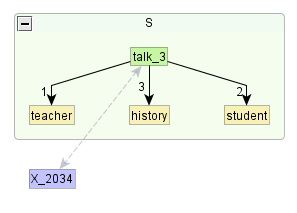
\includegraphics[width=0.4\textwidth, trim = {0cm 0cm 0cm 0cm},clip]{ch6/figs/root.png}
	\caption{Création de la racine à partir du noe{}ud dominant}
	\label{deroulement0}
\end{figure}

\subsection{Sélection du patron de régime dans le lexicon}:
Ensuite, une fois que le noe{}ud dominant est lexicalisé, la règle \emph{actant\_gp\_selection} est déclenchée. Celle-ci permet à GenDR de récupérer les traits encodés dans gp. Puis, à l'intérieur de gp, il y a les traits \texttt{id} et \texttt{dia}. Ces traits sont donc récupérés par la règle et apposé sur le noe{}ud racine. La racine est maintenant contrainte d'utiliser le patron de régime x si la diathèse qu'elle a correspond aux mêmes actants demandés par la structure d'input.

\begin{figure}[htb]
	\centering
	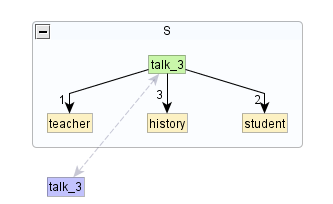
\includegraphics[width=0.4\textwidth, trim = {0cm 0cm 0cm 0cm},clip]{ch6/figs/selectiongp.png}
	\caption{Application de la règle actant\_gp\_selection}
	\label{deroulement1}
\end{figure}

\subsection{Application de la règle actancielle: \emph{actant\_gp\_ijk}}
À l'étape précédente, le noe{}ud \lex{talk\_3} se fait imposer les restrictions suivantes: une paire identifiant de gp et diathèse. Ces traits sont essentiels à l'application des règles actancielles. La règle actant\_gp\_ijk est sélectionnée lorsque la diathèse précise qu'il y a trois actants sémantiques. Il faut aussi que les actants sémantiques que la diathèse précise se retrouve dans la structure sémantique donnée. Sinon, aucune règle actancielle n'est appliquée et la réalisation s'interrompt laissant une racine comme output. 

Ce mécanisme est nouveau puisque dans l'ancienne version de GenDR, le système analysait liaison actancielle individuellement, puis faisait correspondre cet liaison sémantique à une relation syntaxique. Cela se traduisait par la création d'un arc entre la racine et un noe{}ud vide et on y ajoutait des contraintes sur ce noe{}ud simultanément. La version actuelle de GenDR ne fonctionne plus ainsi. Une fois que le gp est sélectionné, on confirme à l'aide du trait dia quel règle actancielle il faudra choisir. Dans notre exemple, ce sera celle-ci puisqu'elle correspond à un gouverneur sélectionnant trois actants.

La règle actant ijk, crée 3 arcs en partance talk\_3 au bout desquels se trouvent des noe{}uds vides sans contraintes. Elle s'occupe aussi du passage des arcs sémantiques à syntaxique. Le patron de régime qui nous concerne est le suivant: \lstinline!gp = { id=NP_V_PP_about_topic_PP_to_co_agent dia=132 }!. On peut y lire que la diathèse précise que le 1 actant sémantique reste le 1er actant syntaxique, mais que le deuxième actant syntaxique est le 3e sémantique et ainsi de suite. Elle crée donc les arcs syntaxiques à partir de ces informations et ils sont vides.

\begin{figure}[htb]
	\centering
	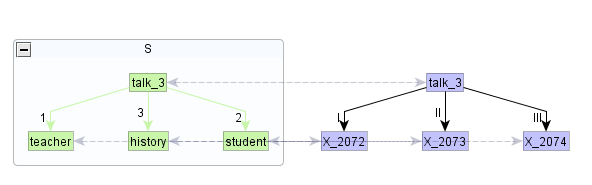
\includegraphics[width=1\textwidth, trim = {0cm 0cm 0cm 0cm},clip]{ch6/figs/actant_gp_ijk.png}
	\caption{Application d'une règle actancielle: actant\_gp\_ijk}
	\label{deroulement2}
\end{figure}

\subsection{Application des contraintes sur les noe{}uds}
Dans l'ancienne version de GenDR, la règle actancielle contraignait aussi les noe{}uds nouvellement créés en syntaxe. Notre système a dû créé une règle séparée de la règle actancielle pour des raisons d'efficacité. Nous avons ainsi créé une règle qui contraints chaque noe{}ud nouvellement créé à partir des informations demandées par le patron de régime pour chaque actant syntaxique. Bref, la règle récupère les restrictions sur les noe{}uds dans le gpcon tel qu'on le voit à la figure \ref{gpexemple}. La règle s'applique donc 3 fois puisqu'il y a trois noe{}uds vides. On a maintenant trois noe{}uds contraints.

\subsection{Lexicalisation des noe{}uds contraints}
Ensuite, on répète une règle de lexicalisation. Dans ce cas il s'agit de \emph{lex\_standard} puisque tous les sémantèmes figurent dans le semanticon et le lexicon. La règle s'applique trois fois car il y a trois noe{}uds. Puis la lexicalisation réussi à chaque fois puisque ces lexèmes satisfont les contraintes imposées aux noe{}uds.
\begin{figure}[htb]
	\centering
	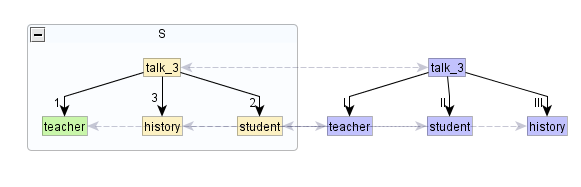
\includegraphics[width=1\textwidth, trim = {0cm 0cm 0cm 0cm},clip]{ch6/figs/lex.png}
	\caption{Applications d'une règle de lexicalisation: lex\_standard}
	\label{deroulement3}
\end{figure}

\subsection{Application de la règle \emph{actant\_gp\_selection}}
Finalement, la règle \emph{actant\_gp\_selection} s'applique encore, mais cette fois-ci pour les lexèmes \lex{teacher},\lex{student} et \lex{history}. Cette règle récupère leurs traits gp.id et gp.dia. Comme ce sont tous des noms communs, ils héritent du gp par défaut de la classe nominale id=NP dia=1 (nous n'avons pas plus d'information sur les patrons de régime des noms compte tenu que VerbNet se spécialisait dans les verbes, mais il existe d'autres ressources parmi celles que nous avions mentionnées qui pourrait combler cette lacune. C'est pourquoi nous n'avons que un gp pour les noms et qu'il est doté d'une diathèse simple permettant de faire la relation complément du nom). encore puisque ces nouveaux noe{}uds lexicalisés déclenchent l'application de la règle. Dès qu'un x a un gp, on va le repêcher, même si on s'en sert pas après. Si l'un d'entre eux avait eu un complément du nom, alors la sélection du gp aurait prouvé son utilité. C'est une application systématique.

Bref, l'application de toutes ces règles à notre input(figure \ref{input-text}) a permi son arborisation. Nous décrirons dans la section suivante le passage vers la structure syntaxique de surface.

\subsection{Lexicalisation de surface}
La première étape est de lexicaliser en surface les lexèmes profonds. Cette règle récupère aussi la partie du discours de surface de l'entrée lexicale. Le procédé est le même que nous avons vu au chapitre \ref{chapgendr}.

\subsection{Règles actancielles de surface}
Une fois que les lexèmes sont réalisés en surface, les règles actancielles de surface sont déclenchées. Trois règles actancielles de surface seront appliquées puisqu'il y a 3 arcs de dépendances (I, II et III) à réaliser. Concrètement, la règle récupère la valeur du trait \texttt{rel}. 

Donc, la règle synt\_subj est déclenchée et le système récupère l'information sur l'actant syntaxique qui possède le trait texttt{rel}. Comme nous avons choisi l'arborisation à partir du gp \emph{NP\_V\_PP\_to\_co\_agent\_PP\_about\_topic}, le système récupère l'information suivante: \lstinline! I={rel=subjective dpos=N}!. Le produit est le changement d'étiquette de la relation pour la valeur \texttt{subjective}.

Simultanément, la règle \emph{synt\_actant\_prep} est déclenchée une première fois pour faire la correspondance entre l'arc syntaxique qui lie \lex{talk\_3} et \lex{history}. La règle récupère ainsi le code suivant: \lstinline! II={rel=oblique dpos=N prep=about}!. Cela signifie que l'actant syntaxique II correspond à la relation \texttt{oblique} en RSyntS. Cette règle est déclenchée car l'un des actants syntaxiques s'expriment en syntaxe de surface à l'aide d'une préposition (une lexie fonctionnelle). Cela a pour incidence que le noe{}ud où profond de \lex{history} se scinde en deux afin que la préposition \lex{about} face le pont entre le verbe et l'objet indirect qu'il sélectionne. Ce phénomène est illustré par la figure~\ref{deroulement4}. 

Cette règle se déclenche une seconde fois pour traiter l'actant syntaxique III \lex{students}.

\subsection{Règles des déterminants}
Finalement, la règle det\_def réalise les déterminants qui doivent apparaître en syntaxe de surface. Ceux-ci correspondent aux traits que nous avions encodés dans l'input de départ. Seul \lex{teacher} et \lex{student} gouverneront des déterminants puisque leurs représentations sémantiques demandaient que les noe{}uds soit définis d'une certaine manière en syntaxe de surface. La règle de déterminant réalise \lex{the} lorsque c'est défini et \lex{a} lorsque le noe{}ud est marqué comme indéfini. Il s'agit d'une règle propre à l'anglais.
\begin{figure}[htb]
	\centering
	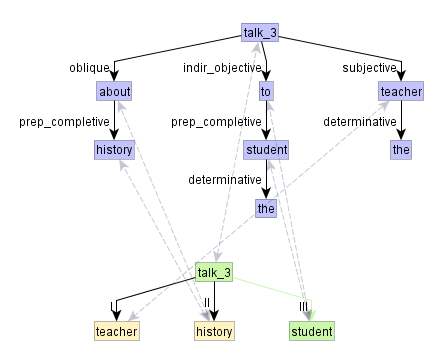
\includegraphics[width=0.5\textwidth, trim = {0cm 0cm 0cm 0cm},clip]{ch6/figs/ssynt.png}
	\caption{Applications des règles actancielles et réalisation des lexies fonctionnelles}
	\label{deroulement4}
\end{figure}
Cela met fin à notre section implémentation. Nous passerons donc à la phase d'évaluation pour vérifier si notre système performe tel que nous l'avions prévu.

\section{Évaluation}
Avant d'entrer dans le vif du sujet, il serait pertinent de faire un bref retour sur les méthodes d'évaluation en \ac{GAT}. \cite{ReiterInvestigationValidityMetrics2009} expliquent qu'il y existe trois types classiques d'évaluation. Ils nomment d'abord la méthode d'évaluation qui se base sur l'exécution d'une tâche en utilisant les textes génénés automatiquement. Ils nomment aussi la méthode d'évaluation humaine. Et finalement, ils parlent des méthodes métriques (automatiques). \cite{ReiterBuildingNaturalLanguage2000} s'étant penché plus tôt sur la question de la validité des méthodes d'évaluation automatiques, ils étaient en faveur d'une évaluation faite par des humains. Toutefois, environ une décennie plus tard, \cite{ReiterInvestigationValidityMetrics2009} remarquaient que les méthodes d'évaluation automatiques se faisaient de plus en plus populaires. Notamment, la méthode BLEU qui avait été développée, à la base, pour les systèmes de traductions automatiques. Nous ferons donc un bref survol de ces méthodes pour décider laquelle se prête le mieux à notre expérience.

BLEU a été créé à la base pour évaluer les rendements des traductions automatiques. Il s'agissait de comparer des outputs d'un système de traduction automatique à un ensemble de traductions humaine (servant de point de référence). Comme la traduction automatique et la génération automatique comportent toutes les deux l'aspect automatique, des chercheurs comme (Langkilde 2002; Habash 2004) ont estimé que la \ac{GAT} bénéficierait de cette méthode d'évaluation. Toutefois, lors de son passage à SemEval2017, FORGe a notamment été évalué par des méthodes métriques et \cite{DBLP:conf/semeval/MilleCBW17} ont fait une brève critique de cette méthode. Ils soulignent que BLEU évalue effectivement bien la couverture, mais comporte des lacunes pour analyser la qualité de chaque output. Leur système avait un score au dessus de la moyenne pour ce qui était de l'évaluation humaine, mais avait reçu un score plus faible pour selon la méthode BLEU. Ils expliquent ce décalage en mentionnant que FORGe mettait de l'avant la qualité de ses outputs par rapport à la quantité. De sorte que ce système filtre à deux reprises les constructions fautives ou potentiellement fautives. (Scoot et Moore, 2007) donnaient aussi quelques mises en garde de la méthode BLEU en précisant qu'elle n'évalue pas toujours correctement des propriétés linguistiques cruciales.

Les méthodes d'évaluation basées sur l'exécution d'une tâche à l'aide de textes générés automatiquement sont assez courantes selon \cite{ReiterInvestigationValidityMetrics2009}. Ces auteurs estiment qu'il s'agit de la méthode qui évalue le mieux le contenu des réalisations d'un système de \ac{GAT}. Toutefois, ils nous mettent en garde que c'est malheureusement la méthode la plus coûteuse en termes de temps et de ressources. En résumé, plus l'output est lisible et clair, plus hautes sont les chances que la tâche soit réalisée rapidement et correctement. Cette méthode n'est pas toujours facile à mettre en place car il faut trouver des participants prêt à donner de leur temps pour lire les rapports générés et effectuer une tâche correspondate. 

Finalement, il y a l'évaluation humaine, plus simple à faire que la méthode à base de tâche, mais plus lente que la méthode automatique. Toutefois, cela reste une méthode très populaire dans le domaine. Il s'agit de coter les outputs en fonction de leur performance à produire des phrases syntaxiquement et sémantiquement acceptables au bon jugement d'un évaluateur.

Considérant ces trois méthodes, nous devons en exclure deux: celle qui est basée sur une tâche et la méthode automatique. D'abord notre système ne réalise pas du texte dans un but précis. On n'a pas de tâche à effectuer pour tester la validité des réalisations. De plus, nous n'avions ni le temps, ni les ressources pour entreprendre ce type d'évaluation. Ensuite, nous ne pouvons pas utiliser la méthode automatique car notre système génère des arbres de dépendances de surface. Les systèmes utilisant la méthode automatique comparent des chaînes de caractères (des réalisations de surface où les textes sont linéarisées et morphologisés). Il nous est donc impossible de comparer nos arbres syntaxiques de surface avec du texte. Il ne reste qu'une méthode d'évaluation s'offrant à nous et c'est celle faite par des humains basée sur nos jugements.

\subsection{Mise en place de l'évaluation}
Pour procéder à l'évaluation de notre système, nous avons utilisé les outputs du script \ref{structurepython} (voir le chapitre \ref{python}). Ceux-ci étaient des structures sémantiques vides dépourvues de prédicats et d'arguments. Il n'y avait que le code pour encadrer le graphe et le texte à reproduire sémantiquement. Nous avons comblé les 978 structures vides en y encodant les unités et relations sémantiques qui correspondaient à l'énoncé. La tâche est simple, nous passerons ces structures sémantiques en input à notre système et nous évaluerons les réalisations produites.

Comme nous avions une quantité limité de temps, nous avons décidé de prendre un échantillon des 978 strucutres sémantiques. Nous en avons choisi 75 aléatoirement. Parmi celles-ci, 25 ont servi à une partie développement précédent la phase d'évaluation comme telle. Ces 25 structures ont été passées au système afin de voir quels sont les problèmes immédiats que nous pouvons réglés sans vérifier si la qualité des arbres produits. Cette phase de développement nous a permi de constater qu'une bon nombre de nos inputs comportaient des problèmes. Nous avons donc noté le type de problème que les inputs comportaient afin de corriger le tir pour la partie évaluation. La partie de développement nous a aussi permi de constater que certains lexèmes appartenant à des PDD différentes apparaissaient en double dans notre dictionnaire. Autrement dit, le verbe \lex{work} et le nom \lex{work} ont la même forme, le système ne sait pas comment les différencier. Cela a donc une incidence sur la réalisation puisque le système construit l'arbre syntaxique à partir du premier lexème qu'il récupère. Donc si nous avions besoin du verbe dans l'arbre et que le système choisi le nom, la réalisation échouera nécessairement. C'est pourquoi nous avons procédé à un filtrage massif de ces cas. Nous les avons réglé en créant une entrée sémantique dans le semanticon qui contiendra les deux entrées lexicales: une version verbale et une version nominale. Elles seront distinguées ainsi dans le semanticon: \lstinline! work { lex = work_n  lex= work_2} !. Bref, nous n'avons pas analysé en profondeur la nature des générations à cette étape, nous voulions seulement répertorier et corriger les problèmes de surface. 

Ensuite, nous avons passé au peigne fin chacun des inputs qui seront évalués. Nous nous sommes assurés que les problèmes d'entrées lexicales répertoriés dans la partie développement étaient corrigés en vue de l'évaluation. Finalement, nous avons pu procéder à la phase de tests. Nous avons testé les 50 structure sémantiques restantes. Pour ce faire, nous avons développé un script qui générait automatiquement toutes les représentations visuelles et textuelles des passages RSem-RSyntP et RSyntP-RSyntS. La partie visuelle permettait de regarder les différentes constructions d'arbres rapidement pour voir lesquelles étaient des réussites ou des échecs. La partie textuelle nous permettait de voir les informations sur les noe{}uds. Par exemple, quel était le patron de régime sélectionné pour cette arborisation ou alors, quelle était la diathèse sélectionnée, ou la partie du discours demandée par le noe{}ud, etc. Ces informations ne sont pas explicitées dans le format graphique de présentation des outputs. 
                              
\subsection{Le rappel}

Nous avons évalué le rappel ainsi:\[\frac{\text{nb str attendues qu'on peut générer}}{\text{nb str attendues}}\]. Cette méthode d'évaluation produit un rappel de 62\%. Ce score se situe au-dessous de nos attentes. Mais il est expliqué par plusieurs facteurs cruciaux dont la majorité peut être corrigée en peu de temps. \draft{entre le 20 et le 30 je vais refaire les calculs avec les corrections pour voir qu'est-ce que ça aurait donné dans le cas échéant.}

D'abord, il y a les erreurs d'encodage qui ont su échapper aux mailles du filet lors de notre filtrage post-développement. Il y avait très peu d'erreur dans l'input sémantique. Nous en avons relevé un seule. Il s'agit de l'emploi d'une mauvaise forme d'un verbe. Nous avons pris grill\_1 et il aurait fallu prendre grill\_3. L'utilisation d'une mauvaise acception d'un verbe mène à l'impossibilité de récupérer le bon patron de régime. En termes d'erreurs humaines, certaines se sont glissées dans les dictionnaires à notre insu. Notamment, une diathèse manquante pour un patron de régime donné. Cela mène à l'impossibilité de réaliser le gp. Ou alors, l'oubli d'une préposition dans une actant syntaxique. Cela fait en sorte qu'en surface, la phrase n'est pas celle qu'on attendait.

Les classes par défaut ont aussi leur lot de problèmes. Effectivement, nous avons dû créer une classe \texttt{quote} pour les patrons de régime qui sélectionne des paroles (Ex: Helen told Ellen "leave the room"). Toutefois, une erreur s'est probablement glissée dans l'encodage de cette classe et le système n'a pas pu la réaliser lors de l'arborisation. Nous avons aussi eu un problème avec les classes qui sélectionnent certaines prépositions. Le système n'est pas capable de récupérer cette préposition dans la classe par défaut, ce qui empêché de réaliser la phrase souhaitée. 

Nous avons eu beacoup de problèmes de rappel lié aux manque de données de la part de VerbNet. Effectivement, il y eut quelques cas de verbes utilisés dans les phrases exemples de VerbNet qui ne figuraient pas dans leur propre dictionnaire verbal. Par le fait même, les patrons de régime associés à ces verbes ne sont pas encodés. Cela mène à l'impossibilité de générer l'arbre qu'on se serait attendu de voir. beg, believe. C'était souvent le cas lorsque la phrase exemple contenait deux verbes. Comme on n'a pas les informations requises pour process le second verbe (diathèse et gp) l'arbre que nous pensions généré ne sera jamais retrieve par GenDR. 

De plus, parmi les problèmes qui nous sont hérités de VerbNet, il y aussi eu quelques cas où la structure sémantique de l'input demandait un patron de régime Y de la part du prédicat, mais que ce patron de régime ne figurait pas parmi la liste de gps de la classe associée à ce verbe. Ou bien he backed out of going  (go\_2: n'avait pas le gp pour réalsier on the trip)

Il y aussi des problèmes due à des incompatibilités sémantique-syntaxe entre VerbNet et la TST. Effectivement, nous n'avons pas tenté de créer une struture sémantique pour qu'elle plaise au patron de régime donné par VerbNet. Cela fait en sorte que quelques des tests allaient nécessairement échouer. Par exemple, la phrase \form{Tom jumped the horse over the fence} est régie par le verbe jump\_2 qui est exprimé par le gp suivant: \lstinline!gp = { id=NP_V_NP_PP_SPATIAL_location dia=123 }!.Les trois actants sémantiques étant \sem{Tom} \sem{horse} et \sem{fence} selon VerbNet. Toutefois, nous considérons que dans ce scénario, le verbe \lex{jump} en surface exprimerait plutôt \sem{faire sauter}. Il existe une fonction lexicale permettant ce genre de situation, mais nous ne l'avons pas encodé dans cette version de VerbNet puisque nous ne touchons pas aux fonctions lexicales. Nous avons noté d'autre cas d'incompatiblités théoriques lors de la phase de développement. 

Nous avons relevé beaucoup de cas d'utilisation de verbe support en surface ('X took a flight' ). Le gp utilisé pour take a flight est bon en soi, mais la représentation sémantique de take est flight ne devrait pas faire appel au gp de take, mais plutôt au gp de flight qui encode les fonctions lexicales (verbe support). et on ne perdrait pas le sens. le \sem{fly} incorpore les lexicalisations \lex{fly} et  \lex{flight}. Took est réalisé comme verbe support en récupérant la fonction lexicale encodée sous \lex{flight}. Nous avons aussi relevé d'autres types de collocations dont X  slept the sleep of the dead. Dans ce cas \form{the sleep of the dead} est une expression figée qui signifie une intensité. Elle modifie le verbe sleep. VerbNet laisse sous-entendre que sleep sélectionne un objet direct qui lui sélectionne un complément du nom. Mais en fait, il ne s'agit que d'un verbe modifié par un intensificateur.

Finalement, le dernier problème qui a le plus affecté le rappel est la défectuosité du mécanisme d'héritage des gps entre les classes dominées et les classes dominantes. Il s'agit du mécanisme dont nous vantions les mérites au début du chapitre. Concrètement, il s'agit d'un moyen qui fait en sorte qu'une class x pointe vers une classe y et hérite des traits encodés dans la classe y. Mais il se trouve que le mécanisme d'héritage des traits fonctionne partiellement. 

Tel que présenté dans le début du chapitre, les unités lexicales pointent vers des classes verbales, une classe verbale peut pointer vers une autre classe verbale, et les classe verbales non-dominées pointent vers la classe par défaut \texttt{verb}. Celle-ci donne les traits dpos=V et spos=verb à tous les lexèmes pointant vers des classes verbales. L'héritage de ce trait est réussi à travers les classes dominées et dominantes car le lexème de surface contient les traits. C'est pourquoi nous disons que le mécanisme fonctionne partiellement. Mais les patrons de régime ne semblent pas se transmettre d'une classe dominante à une classe dominée. Il semblerait que les traits \texttt{id} et \texttt{dia} qui sont encodés dans le trait \texttt{gp} ne sont pas transmis. Ce problème semble provenir de MATE qui n'est pas capable de transmettre l'héritage d'un trait à l'intérieur d'un autre trait. Pour mieux illustrer le concept, nous prendrons le cas de \form{Steved tossed the ball from the corner to the garden.}. Le sémantème \sem{toss\_3} pointait vers la classe \texttt{throw-17.1-1} qui est une classe dominée par "throw-17.1" qui est domineé par "throw-17.1". Cependant le patron de régime dont nous avions besoin pour réaliser la phrase souhaitée se trouvait dans le régime de la classe mère "throw-17.1". GenDR n'a donc pas été capable d'aller chercher les traits id et dia. Mais il a été capable de réaliser la racine de l'arbre avec le lexème \lex{throw\_3} en héritant du trait dpos de la classe par défaut \texttt{verb}.

Pour pallier à ce mécanisme d'héritage deffectueux, nous pourrions directement implémanter tous les gps des classes dominantes dans les classes dominées. Ainsi on garde l'architecture pensée de VerbNet où les classes héritent des patrons des autres classes. Le défaut de cette solution est que notre dictionnaire sera saturé d'information puisqu'il existe énormément de sous-classe. Toutefois, cette solution est facilement adaptable puisque nous avons encore les scripts Python ayant servi à extraire les patrons de régime et à créer le lexicon. Nous n'avons qu'à modifier le script pour que chaque sous-classe hérite explicitement des gps des classe qui les domine. Évidemment, cela aurait aussi un impact direct sur la précision, puisqu'on a plus de chance de générer une erreur si plusieurs gps sont disponibles.

\subsection{Précision}

Nous avons noté la précision de cette manière:\[\frac{\text{nb str correctes}}{\text{nb str générées}}\]. Cela nous donne une précision de 77\%.

Les erreurs humaines que nous avions mentionnées pour le rappel ont généralement un impact sur la précision. Par exemple, en mettant la mauvaise désambiguisation d'un verbe dans l'input, alors les patrons de régime utilisés pour réaliser la phrase ne seront pas les bons. Cela peut générer de bonnes phrases, si par chance un bon gp s'y trouve. Mais on a vu que cela pouvait générer des phrases incongrues: \form{She grilled the steak on me} ou \form{She grilled the steak in me}.

Les erreurs de VerbNet affectent aussi la précision de l'output négativement. Lorsqu'un verbe utilisé dans l'exemple n'est pas répertorié par VerbNet. Le système utilise ses règles de secours de lexicalisation et va tout de même tenter de réaliser quelque chose. C'est le cas d'une phrase ayant le verbe \lex{do} pour \form{I begged her to do it}. Comme GenDR n'a pas hérité de l'entrée que VerbNet aurait dû avoir, le système a tenté diverses réalisations. Certaines d'entre elles échoueront, mais d'autres seront réalisées en surface. C'est le cas de \form{I begged her for the do.}. Dans ce cas, GenDR a supposé que c'était possiblement un nom. Et comme il existait un patron de régime de \lex{beg} permettant cette construction, alors le système a réalisée cette incongruité. Nous avons relevé d'autres cas similaires dans notre évaluation.

Les informations extraites de VerbNet nous ont aussi fait réaliser des phrases quasi-correctes mais bizarres. C'est une conséquence des patrons de régime qui permettent 2 à 4 prépositions différentes pour la réalisation d'une actant syntaxique en surface. Le système va donc générer deux arbres différents corrects. Chacun d'entre eux aura une préposition différente pour l'actant concerné, mais généralement seule l'une d'entre elle génère une phrase grammaticale. Ainsi, GenDR a généré les phrases \form{The doctor cured pat of pneumonia} et \form{The doctor cured pat out of pneumonia}. La deuxième est un arbre bien construit, mais dont la sémantique est fautive.

Un autre type d'erreur de précision provient de la manière dont GenDR génère les arbres. Tel que nous l'avons vu plus tôt, le système crée x nombres de racines pour un input où x est le nombre de patron de régime inclu pour une classe verbale. 

Ensuite, on sélectionne les gps et on vérifie que la diathèse permet l'appplication du gp sélectionné. C'est là que le problème prend forme. GenDR peut ainsi sélectionner un gp fautif qui respecte la diathèse et les contraintes sur le noe{}ud. Mais, il est possible que l'arborisation échoue parce que l'un des actants syntaxiques choisi contient une préposition qui rendra la phrase agrammaticale. Concrètement pour régler ce problème, il faudrait revoir l'application de nos règles. Par exemple la phrase \form{The street gushed}. Rien dans notre système nous empêchait de réaliser cette forme fautive.

\subsection{Synthèse de l'évaluation}

\draft{Est-ce que c'est pertinent que je parle de la f1 ? Elle est de 69\%}
\draft{Est-ce que j'ai besoin de faire un retour sur ce qui a été dit ? Ou bien j'en parle dans ma conclusion finale}

Ce qu'on retire de tout cela sont deux problèmes majeurs. Le mécanisme d'héritage qui fonctionne partiellement avec l'architecture présente qui nuit au rappel.

De plus, il faut aussi tenir compte du fait que nous avons testé sur 5\% des structures d'input. Mais nous pensons que c'est un 5\% significatif. Les mêmes erreurs revenaient souvent dans l'analyse des résultats.

